\section{법선 벡터(Normal Vector)}

\subsection{배경과 역사}
법선 벡터(Normal Vector)는 기하학 및 물리학에서 중요한 개념으로, 곡선이나 표면에서 특정 점에서 수직 방향을 나타내는 벡터입니다. 이 개념은 18세기 수학자들이 곡선 및 곡면의 성질을 연구하면서 등장했으며, 현대에 이르러 컴퓨터 그래픽스, 물리학, 기계 학습 등 다양한 분야에서 중요한 역할을 합니다.

\vspace{1\baselineskip}
\noindent 특히, 법선 벡터는 3D 그래픽스에서 빛의 반사와 표면의 입체감을 계산하는 데 필수적인 요소로 자리잡았습니다. 물리학에서는 힘의 방향을 정의하거나 충돌에 따른 반사 및 굴절을 설명할 때 법선 벡터가 사용됩니다.

\subsection{정의와 목적}
법선 벡터는 평면, 곡선 또는 곡면의 한 점에서 그 표면에 수직인 벡터로 정의됩니다. 2차원에서는 직선의 기울기에 수직인 벡터로, 3차원에서는 평면이나 곡면에 수직인 벡터로 정의됩니다. 수학적으로, 주어진 곡면의 점에서 법선 벡터는 해당 점에서의 접선 벡터에 수직입니다.

\vspace{1\baselineskip}
\noindent 법선 벡터의 주요 목적은 표면에서의 수직 방향을 나타내는 것이며, 이를 통해 빛의 반사, 물리적 충돌 등 다양한 물리적 현상을 설명할 수 있습니다.

\subsection{연산의 이유와 유용성}
법선 벡터는 다음과 같은 이유로 유용하게 사용됩니다:
\begin{itemize}
  \item \textbf{3D 그래픽스와 조명}: 3D 그래픽스에서 법선 벡터는 빛의 반사와 그림자를 계산하는 데 매우 중요합니다. 광선이 표면에 닿을 때 법선 벡터를 통해 표면이 빛을 어떻게 반사할지를 결정할 수 있습니다. 법선 벡터는 또한 표면의 윤곽과 질감을 결정하여 3D 모델의 입체감을 형성합니다.

        \vspace{1\baselineskip}
        \noindent \emoji{shopping} e.g. 컴퓨터 그래픽스에서 표면 법선 벡터를 사용하여 물체에 빛이 닿는 각도에 따라 그림자와 반사광을 계산할 수 있습니다. 만약 법선 벡터 \( \mathbf{n} \)이 표면에서 수직으로 설정되면, 광선 \( \mathbf{L} \)과의 내적을 통해 조명 계산이 이루어집니다.

  \item \textbf{물리학에서 힘의 방향}: 물리학에서는 법선 벡터를 통해 충돌이나 힘의 방향을 설명할 수 있습니다. 예를 들어, 물체가 표면에 부딪힐 때 법선 벡터는 반사되는 힘의 방향을 결정하는 데 사용됩니다.

        \vspace{1\baselineskip}
        \noindent \emoji{shopping} e.g. 충돌 시, 법선 벡터는 충돌 후 물체가 튕겨 나가는 반사 방향을 결정합니다. 물체가 표면에 충돌하는 각도와 법선 벡터 간의 관계는 반사 법칙을 따릅니다.
\end{itemize}

\subsection{예시: \( ax + by + cz + d = 0 \)의 법선 벡터}
평면 방정식 \( ax + by + cz + d = 0 \)에서 각 변수 \( x \), \( y \), \( z \)에 대한 편미분은 다음과 같습니다:
\[
  \frac{\partial}{\partial x} (ax + by + cz + d) = a, \quad \frac{\partial}{\partial y} (ax + by + cz + d) = b, \quad \frac{\partial}{\partial z} (ax + by + cz + d) = c
\]
따라서 법선 벡터 \( \mathbf{n} \)은:
\[
  \mathbf{n} = (a, b, c)
\]

\subsection{법선 벡터와 평면의 그래프}
아래는 평면 \( x + 2y + 3z + 4 = 0 \)과 그에 수직인 법선 벡터 \( (1, 2, 3) \)의 3D 그래프입니다.

\begin{center}
  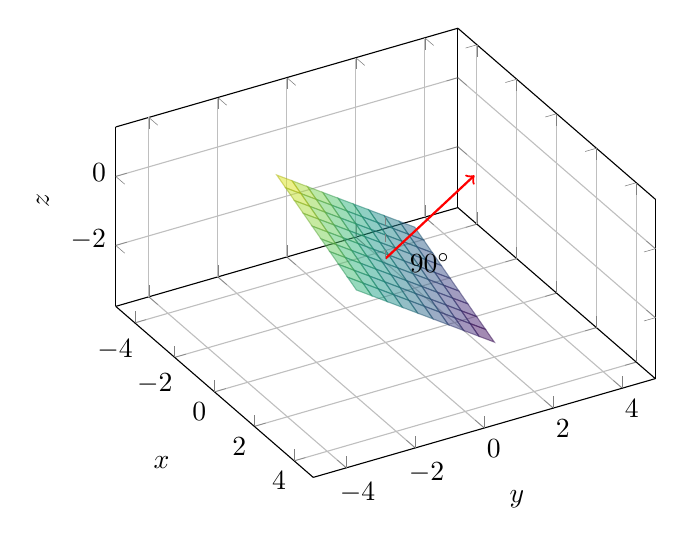
\begin{tikzpicture}
    \begin{axis}[
        view={60}{30},
        xlabel={$x$},
        ylabel={$y$},
        zlabel={$z$},
        domain=-2:2, y domain=-2:2,
        colormap/viridis,
        samples=10,
        grid=both,
        axis equal
      ]
      % 평면의 방정식: x + 2y + 3z + 4 = 0
      \addplot3[surf, opacity=0.5] {-(x + 2*y + 4)/3};

      % 외향 법선. 정확한 법선 벡터 (1, 2, 3) 수정, 시작점과 크기 확인. TODO: 📰 vs. 내향 법선
      \addplot3[->, thick, red] coordinates {(0, 0, -4/3) (1, 2, 1)};

      % 수직선 표시
      \addplot3[dashed, gray] coordinates {(0, 0, -4/3) (0, 0, 0)};

      % 각도 표시
      \node at (axis cs:0.5,1,-1.5) {$90^\circ$};

    \end{axis}
  \end{tikzpicture}
\end{center}

\noindent 여기서, 법선 벡터는 평면에 정확히 수직으로 그려져 있으며, 각도 \( 90^\circ \)를 표시하여 이를 명확히 보여줍니다.

\subsection{비교 | 대조 | 성질}
법선 벡터는 다양한 특수 벡터와 비교하여 독특한 성질을 가집니다. 주요 성질은 다음과 같습니다:

\begin{itemize}
  \item \textbf{직교성(Orthogonality)}: 법선 벡터는 해당 표면의 접선 벡터(tangent vector)와 항상 수직 관계에 있습니다. 이는 법선 벡터가 표면에 대해 직교한다는 것을 의미합니다.

  \item \textbf{단위 벡터(Normalized Vector)}: 일반적으로 법선 벡터는 크기가 1인 단위 벡터로 정규화됩니다. 이는 계산의 간결성을 위해 표준화된 방식입니다.

  \item \textbf{곡면에서의 법선 벡터}: 곡면의 법선 벡터는 매끄러운 곡선 위의 각 점에서 변화하며, 이는 표면의 기하학적 특성을 반영합니다. 이러한 변화는 곡률과 관련이 있으며, 표면의 기하학적 성질을 분석하는 데 사용됩니다.
\end{itemize}

\subsection{응용 | 실제 사례}
법선 벡터는 다양한 실생활 문제와 연관되어 있습니다. 주요 응용은 다음과 같습니다:

\begin{itemize}
  \item \textbf{컴퓨터 그래픽스(Computer Graphics)}: 3D 그래픽스에서 법선 벡터는 표면의 입체감을 결정하는 데 사용됩니다. 빛의 반사, 그림자, 물체의 텍스처를 계산하는 데 필수적입니다. 특히 법선 맵핑(Normal Mapping) 기법을 통해 복잡한 표면의 세부 질감을 보다 현실감 있게 표현할 수 있습니다.

        \vspace{1\baselineskip}
        \noindent \emoji{shopping} e.g. 법선 벡터는 3D 그래픽스 엔진에서 표면의 미세한 디테일을 구현하는 데 사용됩니다. 예를 들어, 물체의 매끄러운 표면을 표현할 때, 법선 맵핑 기술을 통해 더욱 정교한 표현을 할 수 있습니다.

  \item \textbf{물리학(Physics)}: 물리학에서 법선 벡터는 충돌이나 굴절을 계산할 때 사용됩니다. 예를 들어, 공이 벽에 부딪힌 후 튕겨 나가는 방향은 법선 벡터를 기준으로 계산됩니다. 또한, 빛의 굴절과 반사에서 법선 벡터는 스넬의 법칙(Snell's Law)에 따라 빛의 경로를 결정하는 중요한 요소입니다.
\end{itemize}

\subsection{관련 논문 | 참고 자료}
법선 벡터에 대한 더 깊은 이해를 위해 다음과 같은 문헌을 참조할 수 있습니다:

\begin{itemize}
  \item \textit{Foley et al.}, \textit{Computer Graphics: Principles and Practice} – 법선 벡터와 표면 법선에 대한 3D 그래픽스에서의 응용을 포괄적으로 설명합니다.
  \item \textit{Gilbert Strang}, \textit{Linear Algebra and Its Applications} – 선형대수학에서의 법선 벡터의 기초 이론과 응용을 설명합니다.
  \item \textit{David J. Griffiths}, \textit{Introduction to Electrodynamics} – 전자기학에서 법선 벡터가 어떻게 전기장과 자기장 계산에 사용되는지 설명합니다.
\end{itemize}
